%============================================================
%  Capitolo 2 – Learning Representations
%============================================================
\chapter{Learning Representations}
\label{ch:learning-repr}

Questo capitolo affronta una domanda fondamentale: \textit{perché le reti profonde
funzionano meglio di quelle shallow?} La risposta passa per il concetto di
\textbf{rappresentazione}: trasformare i dati grezzi in uno spazio in cui il
problema diventi più facile da risolvere \citep{bishop2024, lecun2021}.

%------------------------------------------------------------
\section{Limiti dei Classificatori Lineari}
\label{sec:linear-limits}

Un \textbf{classificatore lineare} assegna la classe in base al segno di una
combinazione lineare delle feature:
\begin{equation}
  \bar{y} = \operatorname{sign}\!\left(\sum_{i=1}^{N} w_i x_i + b\right).
\end{equation}
Geometricamente, il classificatore partiziona lo spazio in due semispazi
separati dall'iperpiano $\sum_i w_i x_i + b = 0$. Il vettore $\vect{w}$
è la normale all'iperpiano e ne determina l'orientamento; $-b/w_1$ ne fissa
l'intercetta.

\begin{figure}[H]
  \centering
  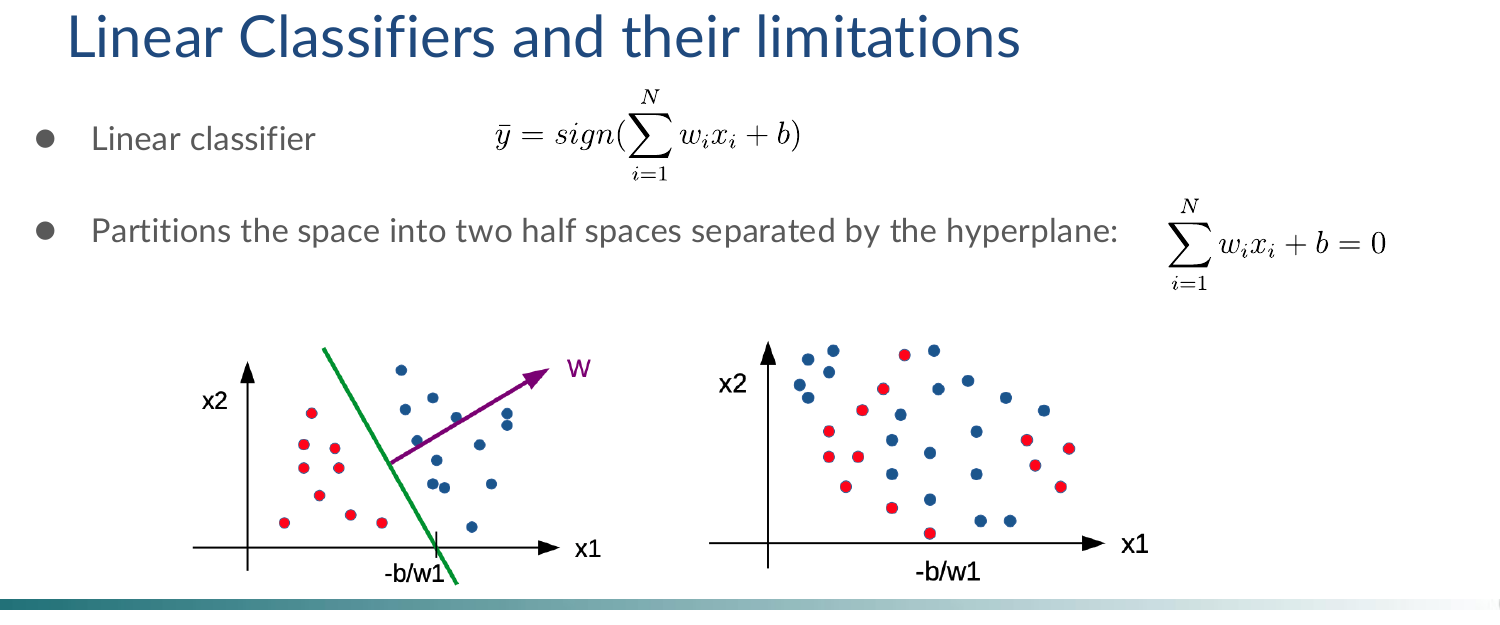
\includegraphics[width=0.88\linewidth]{figures/lr02_linear_classifier.png}
  \caption{Classificatore lineare in 2D. Sinistra: caso separabile linearmente
           -- l'iperpiano (retta verde) divide correttamente le due classi.
           Destra: caso non separabile linearmente -- nessuna retta può separare
           i punti rossi da quelli blu.}
  \label{fig:linear_classifier}
\end{figure}

Il limite fondamentale dei classificatori lineari è formalizzato dal
\textbf{Teorema di Cover (1966)}: la probabilità che una dicotomia casuale
di $P$ punti in $N$ dimensioni sia linearmente separabile tende a zero
quando $P \gg N$.

\begin{figure}[H]
  \centering
  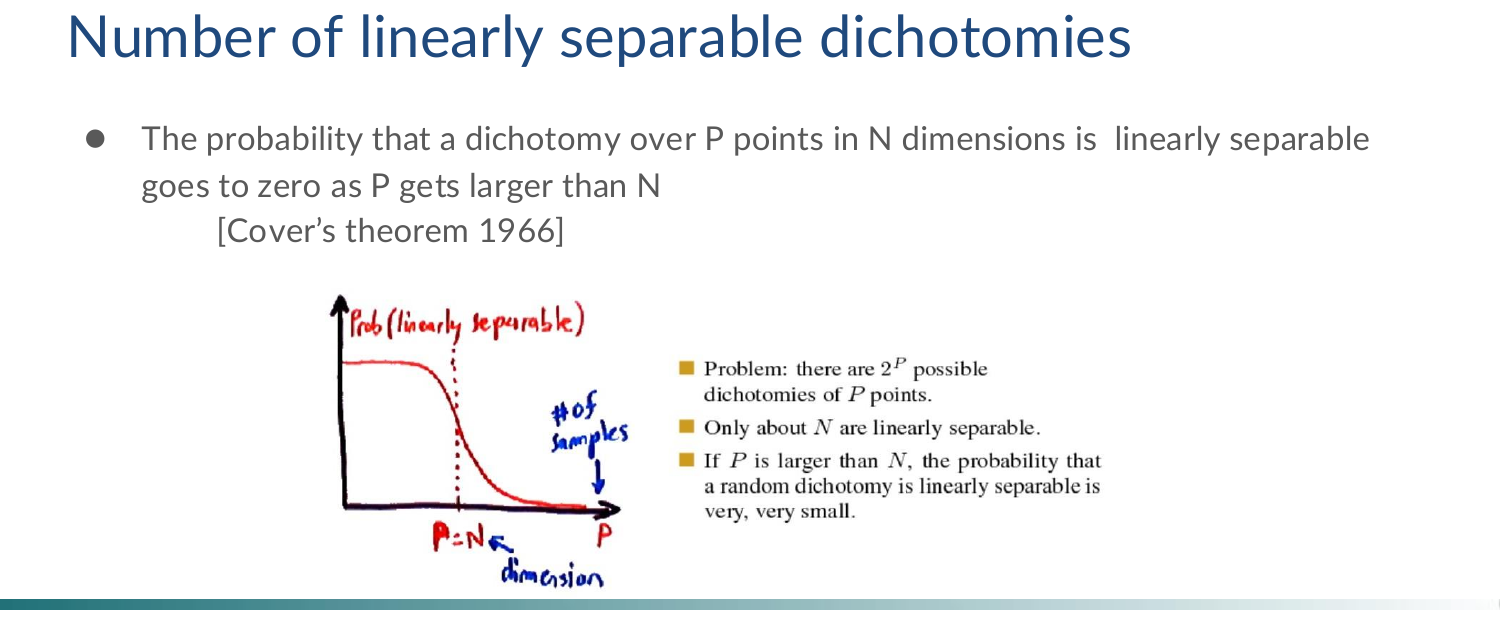
\includegraphics[width=0.75\linewidth]{figures/lr02_cover_theorem.png}
  \caption{Teorema di Cover: la probabilità di separabilità lineare crolla
           bruscamente non appena il numero di campioni $P$ supera la
           dimensionalità $N$. Esistono $2^P$ possibili dicotomie, ma solo
           circa $N$ sono linearmente separabili.}
  \label{fig:cover_theorem}
\end{figure}

In pratica: con $P \gg N$, quasi nessuna dicotomia casuale è linearmente
separabile. Per classificare dati reali complessi, occorre una
\textbf{trasformazione non lineare} che renda il problema separabile.

%------------------------------------------------------------
\section{La Soluzione: Rappresentazioni (Feature)}
\label{sec:solution-repr}

La soluzione è costruire un \textbf{estrattore di feature} che trasformi
l'input grezzo in una rappresentazione in cui un classificatore lineare
possa operare efficacemente. L'estrattore deve essere \emph{non lineare}:
una trasformazione lineare non cambia la separabilità del problema.

\begin{figure}[H]
  \centering
  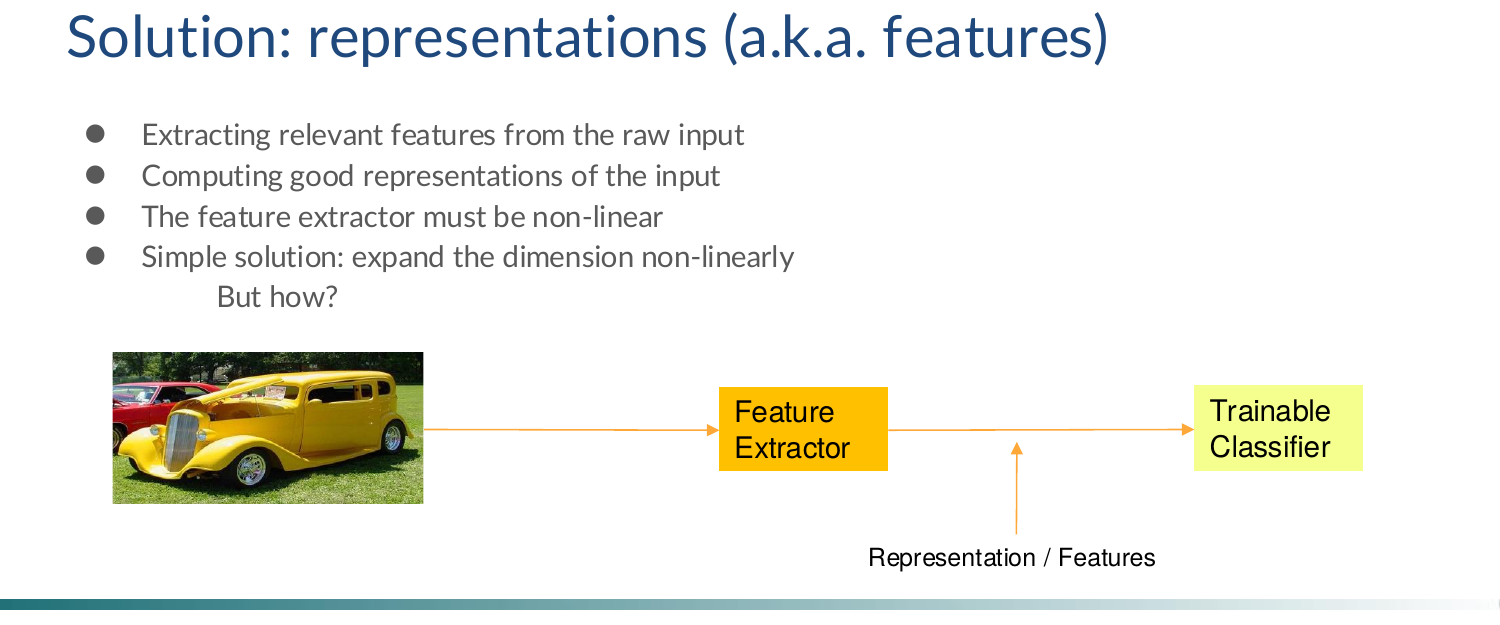
\includegraphics[width=0.80\linewidth]{figures/lr02_solution_repr.png}
  \caption{Soluzione con rappresentazioni: il blocco Feature Extractor
           trasforma l'input grezzo in una rappresentazione/feature; su queste
           opera un classificatore trainable. Nel DL anche l'estrattore è
           addestrato end-to-end.}
  \label{fig:solution_repr}
\end{figure}

Il principio di base è \textbf{espandere la dimensionalità} in modo non
lineare: in uno spazio di dimensione maggiore, punti che erano non separabili
diventano separabili con alta probabilità (per il Teorema di Cover, la
probabilità di separabilità cresce con $N$).

\subsection{Idee per l'estrazione generica di feature}

Esistono diverse strategie ``generiche'' per costruire feature non lineari
\reflecun{W2}:

\begin{itemize}
  \item \textbf{Space tiling}: si suddivide lo spazio di input in regioni e
        si usano indicatori di appartenenza come feature.
  \item \textbf{Random projections}: si proietta l'input su vettori casuali
        seguiti da non-linearità (es.\ ReLU). Alla base dei \textit{reservoir
        computing} e delle \textit{random features} per kernel approximation.
  \item \textbf{Feature monomiali} (cross-products): il feature extractor
        calcola prodotti di coppie (o triple, ecc.) di variabili di input;
        un classificatore lineare su queste feature calcola un polinomio
        dell'input.
  \item \textbf{Radial Basis Functions (RBF)}: feature del tipo
        $\phi_k(x) = \exp(-\|x - c_k\|^2 / 2\sigma^2)$, con centri $c_k$
        fissati o appresi.
  \item \textbf{Kernel machines}: generalizzano le RBF attraverso funzioni
        kernel $K(x^j, x)$; le SVM ne sono l'esempio principale.
\end{itemize}

\subsection{Feature monomiali e limiti}

\begin{figure}[H]
  \centering
  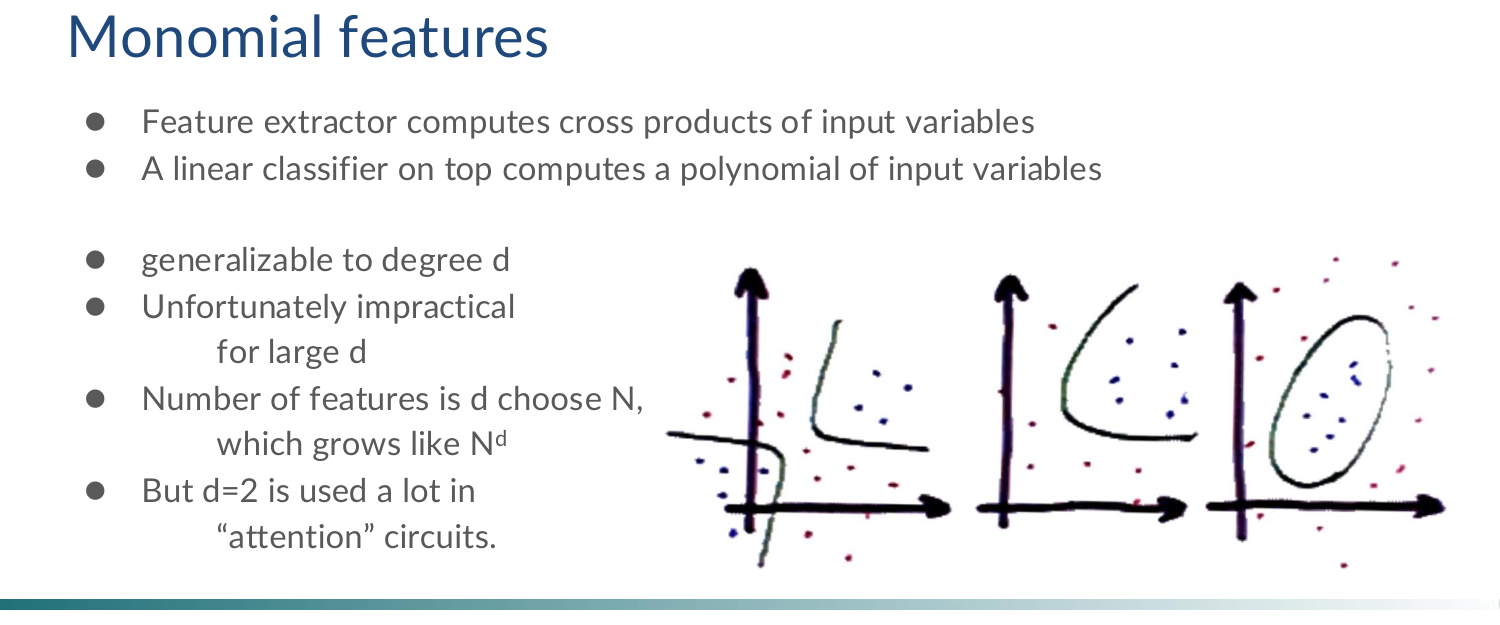
\includegraphics[width=0.82\linewidth]{figures/lr02_monomial.png}
  \caption{Feature monomiali: aggiungendo il termine quadratico $x_1 x_2$
           (o più in generale prodotti di grado $d$) come feature, un
           classificatore lineare può separare pattern che erano non lineari
           nell'input originale -- ad esempio boundary ellittici o a forma
           di C.}
  \label{fig:monomial}
\end{figure}

Le feature monomiali di grado $d$ su $N$ variabili producono
$\binom{N+d}{d} \sim N^d$ feature: questo numero cresce esponenzialmente con
$d$, rendendo il metodo impraticabile per grandi $d$.
Tuttavia, il caso $d=2$ è molto usato nei circuiti di
\textit{attention} (si veda il Cap.\,\ref{ch:basic-arch}), in quanto corrisponde
esattamente alle unità Sigma-Pi.

%------------------------------------------------------------
\section{Reti Shallow vs Reti Profonde}
\label{sec:shallow-vs-deep}

\subsection{Le reti shallow sono approssimatori universali}

Un risultato teorico fondamentale afferma che una rete neurale a 2 layer con
numero sufficiente di unità nascoste può approssimare qualsiasi funzione
continua con precisione arbitraria \refbishop{6}. Lo stesso vale per le
\textbf{Support Vector Machine} con kernel:
\begin{equation}
  G(X,\alpha) = \sum_j \alpha_j K(X^j, X),
\end{equation}
dove il primo layer calcola i kernel $K(X^j, X)$ usando i campioni di
training come template, e il secondo layer è una combinazione lineare con
pesi $\alpha_j$.

\begin{figure}[H]
  \centering
  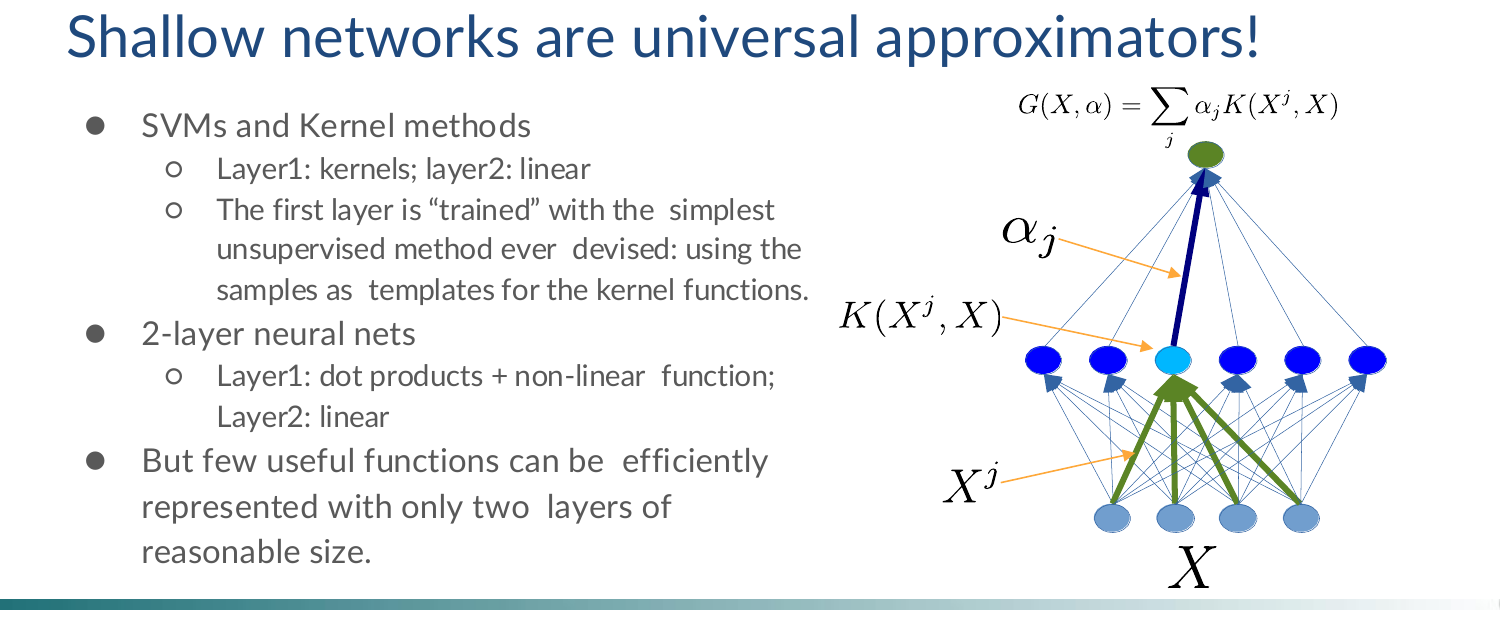
\includegraphics[width=0.80\linewidth]{figures/lr02_shallow_universal.png}
  \caption{Architettura di una kernel machine (SVM): il primo layer calcola
           $K(X^j, X)$ per ogni campione di training $X^j$; il secondo layer
           combina linearmente le attivazioni con pesi $\alpha_j$.}
  \label{fig:shallow_universal}
\end{figure}

\subsection{Perché servono architetture profonde?}

Se le reti shallow sono universali, perché usare reti profonde? Il
\textbf{dilemma del teorico} pone esattamente questa domanda.

\begin{figure}[H]
  \centering
  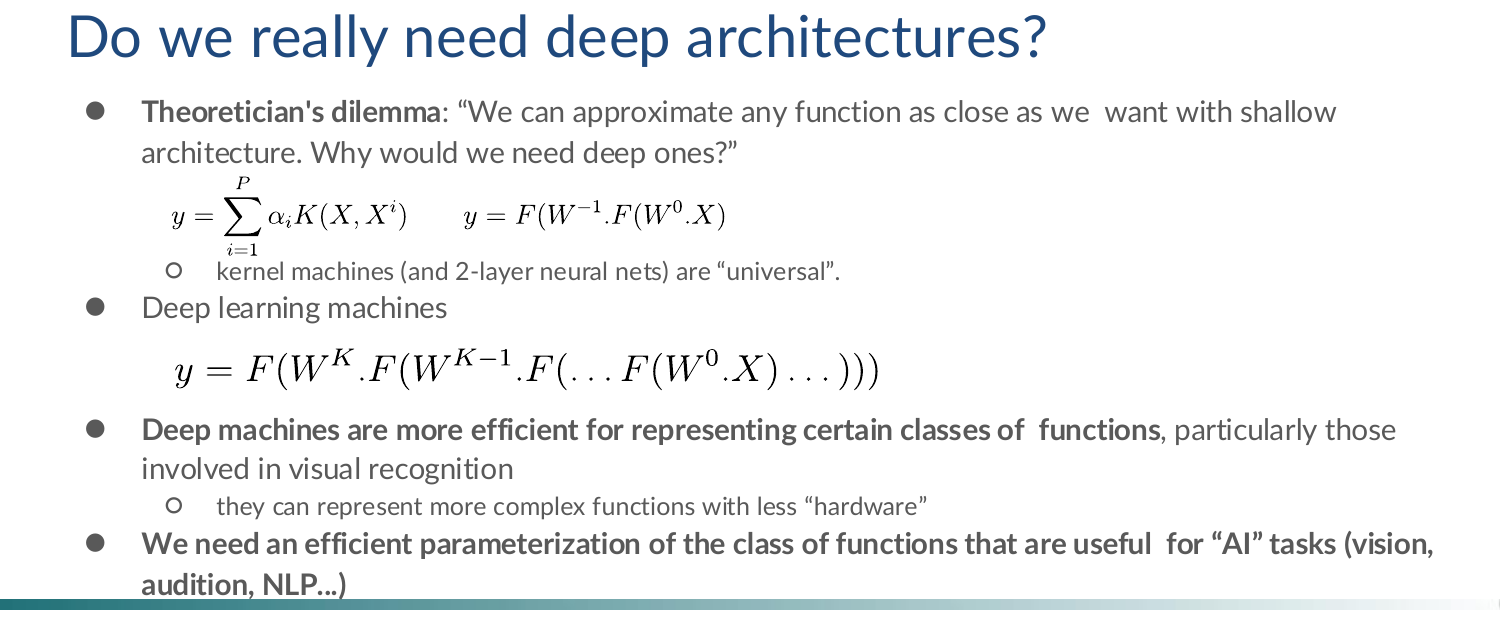
\includegraphics[width=0.88\linewidth]{figures/lr02_deep_vs_shallow.png}
  \caption{Confronto tra reti shallow e profonde: una rete shallow (kernel
           machine o 2-layer net) può rappresentare qualunque funzione, ma
           richiede un numero esponenziale di unità per funzioni complesse;
           una rete profonda $y = F(W^K \cdot F(\ldots F(W^0 \cdot X)\ldots))$
           le rappresenta in modo molto più efficiente.}
  \label{fig:deep_vs_shallow}
\end{figure}

La risposta è nell'\textbf{efficienza della rappresentazione}: le reti
profonde possono rappresentare certe classi di funzioni -- in particolare
quelle coinvolte nel riconoscimento visivo -- con molti meno parametri
rispetto alle reti shallow \citep{bishop2024}. Come argomenta
\citet{lecun2021}, una rete profonda \textit{scambia spazio con tempo}
(o ampiezza con profondità): più layer sequenziali ma meno hardware parallelo.

%------------------------------------------------------------
\section{Invariant Feature Learning}
\label{sec:invariant-features}

L'idea di base per imparare feature invarianti è la seguente
\reflecun{W2}:

\begin{enumerate}
  \item \textbf{Espandere} l'input non linearmente in uno spazio ad alta
        dimensionalità (feature instabili ma discriminative).
  \item \textbf{Aggregare} regioni del nuovo spazio (pooling, proiezione,
        riduzione di dimensionalità) per ottenere feature stabili e invarianti.
\end{enumerate}

\begin{figure}[H]
  \centering
  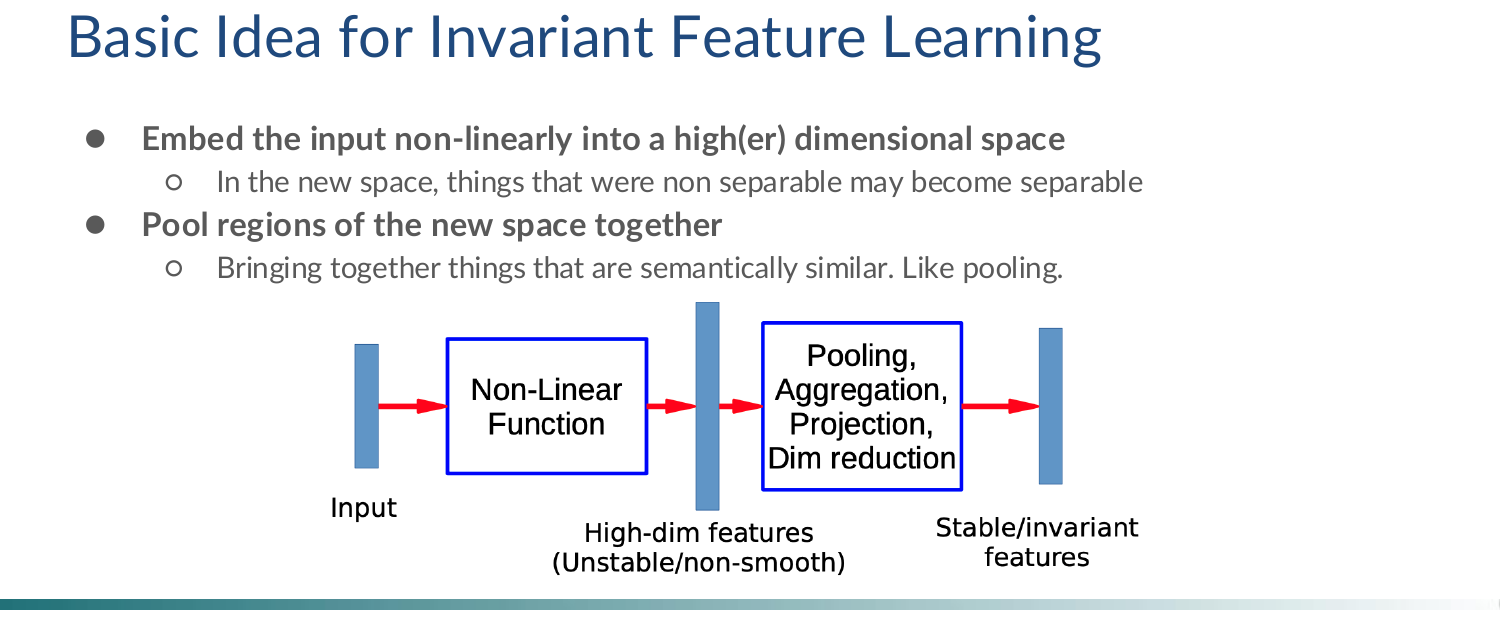
\includegraphics[width=0.82\linewidth]{figures/lr02_invariant_learning.png}
  \caption{Schema dell'invariant feature learning: la funzione non lineare
           espande l'input in feature ad alta dimensione (instabili), che
           vengono poi aggregate tramite pooling/aggregazione/dim.\
           reduction per produrre feature stabili e invarianti.}
  \label{fig:invariant_learning}
\end{figure}

%------------------------------------------------------------
\section{L'Ipotesi del Manifold}
\label{sec:manifold}

\begin{definizione}[Manifold Hypothesis]
I dati naturali vivono in un \textbf{manifold non lineare a bassa dimensione}
immerso nello spazio ad alta dimensione. Le variabili nei dati naturali sono
mutuamente dipendenti, per cui la variabilità intrinseca è molto più bassa
della dimensione nominale.
\end{definizione}

\begin{figure}[H]
  \centering
  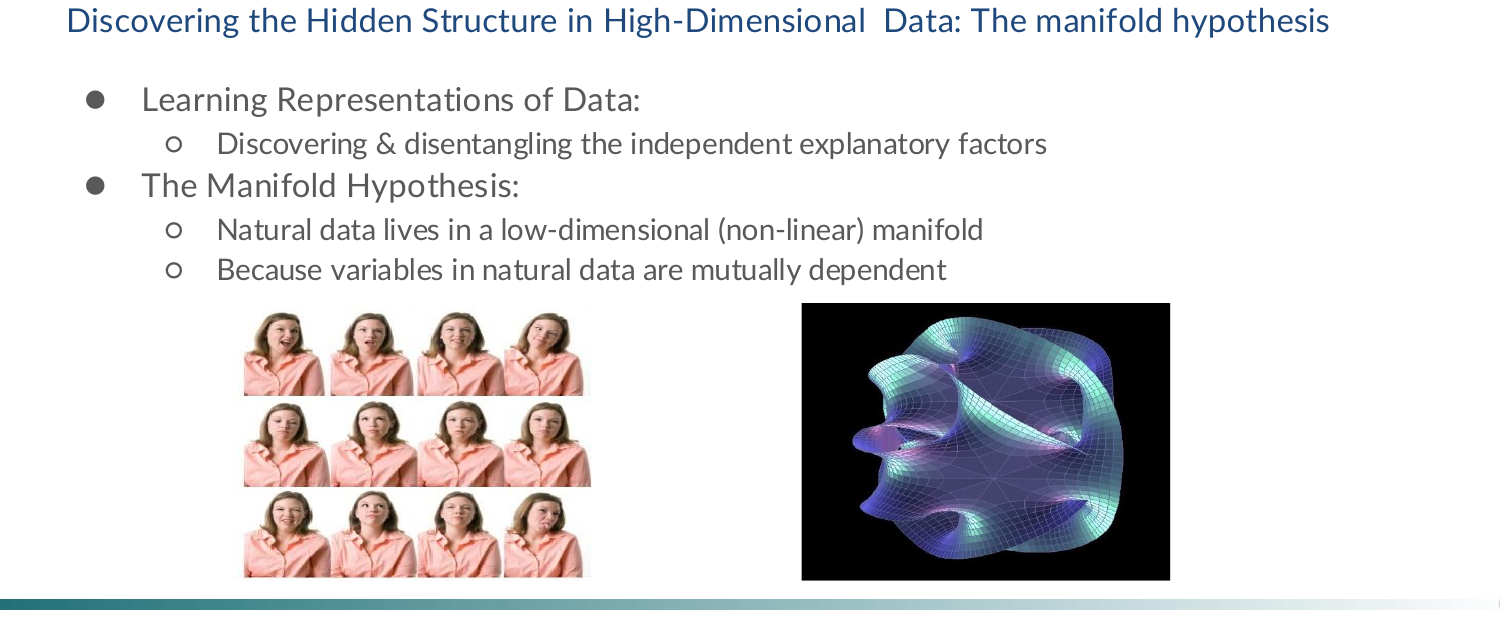
\includegraphics[width=0.88\linewidth]{figures/lr02_manifold_hypothesis.png}
  \caption{L'ipotesi del manifold: le immagini di volti (sinistra) variano
           in espressione, posa, illuminazione -- ma questa variabilità
           appartiene a un manifold a bassa dimensione (destra), non a tutto
           lo spazio dei pixel.}
  \label{fig:manifold_hypothesis}
\end{figure}

\paragraph{Esempio: immagini di volti.}
Un'immagine $1000 \times 1000$ pixel ha $10^6$ dimensioni. Tuttavia un volto
è descritto da soli 3 coordinate cartesiane, 3 angoli di Eulero e meno di 50
muscoli facciali: il manifold delle immagini di un volto ha quindi meno di 56
dimensioni effettive.

\begin{figure}[H]
  \centering
  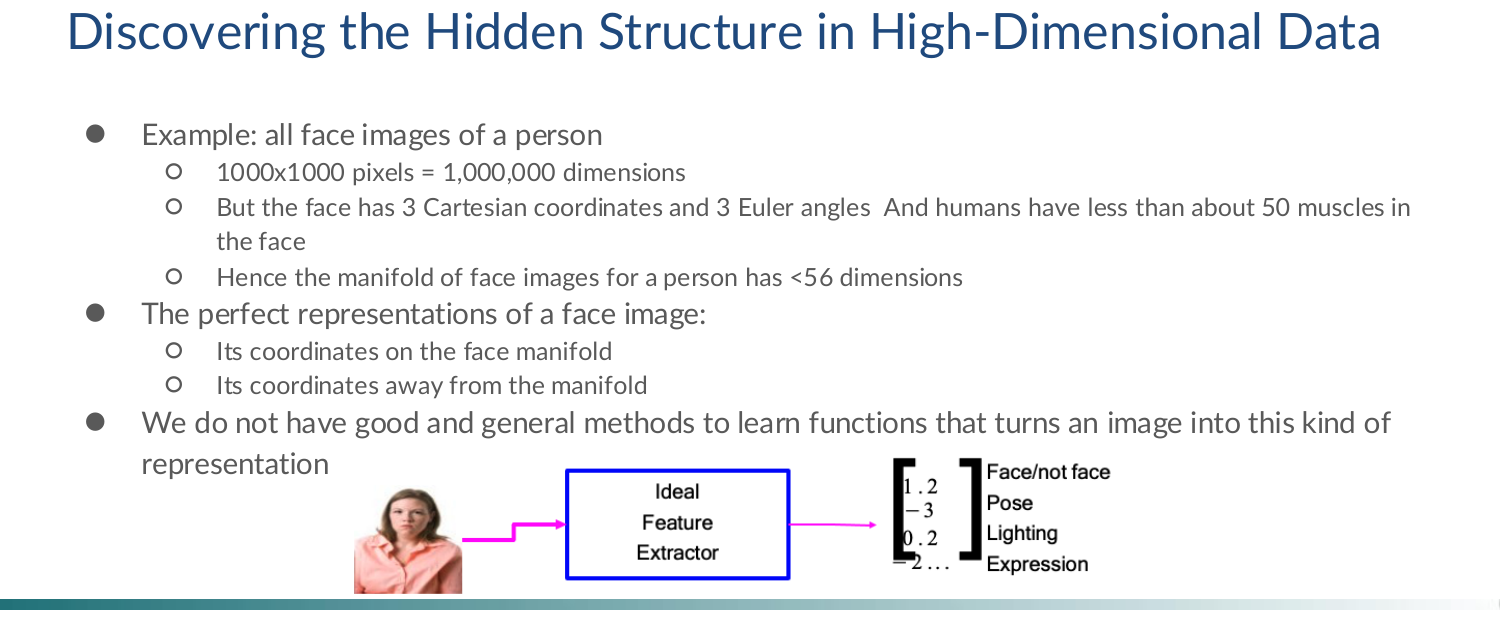
\includegraphics[width=0.82\linewidth]{figures/lr02_face_manifold.png}
  \caption{La rappresentazione ideale di un'immagine facciale ne estrae le
           coordinate sul manifold (pose, lighting, expression\ldots) come
           vettore compatto. Non disponiamo ancora di metodi generali per
           imparare questa funzione.}
  \label{fig:face_manifold}
\end{figure}

%------------------------------------------------------------
\section{Disentangling e Apprendimento delle Rappresentazioni}
\label{sec:disentangling}

L'obiettivo del \textbf{representation learning} è scoprire e
\emph{disintrecciare} (disentangle) i fattori di variazione indipendenti
che generano i dati.

\begin{figure}[H]
  \centering
  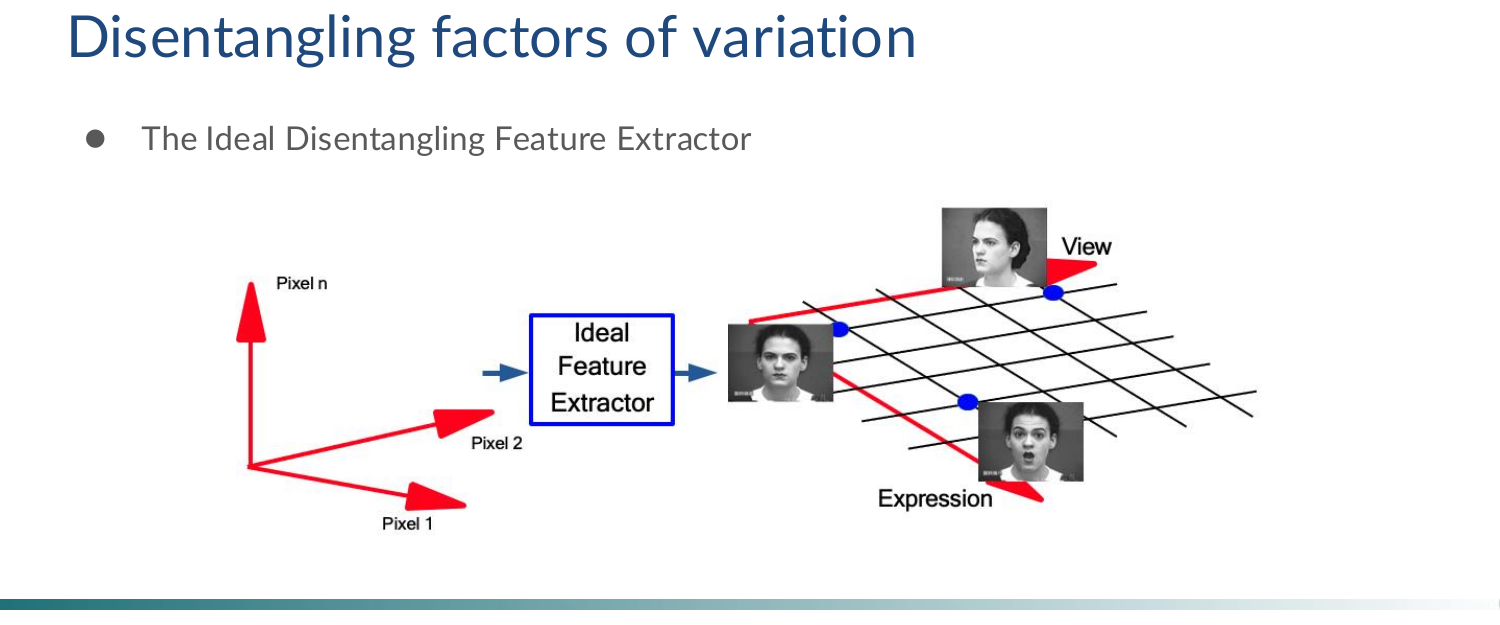
\includegraphics[width=0.88\linewidth]{figures/lr02_disentangling.png}
  \caption{L'ideal feature extractor mappa lo spazio dei pixel (sinistra)
           nel manifold dei volti (destra), dove le coordinate corrispondono
           a fattori interpretabili come ``view'' (punto di vista) e
           ``expression'' (espressione). Ogni punto blu nel manifold
           corrisponde a un'immagine specifica.}
  \label{fig:disentangling}
\end{figure}

Un esempio concreto di manifold appreso è mostrato nel lavoro di
Hadsell et al.\ (CVPR 2006): immagini di aeroplani in diverse rotazioni
sono disposte su una curva chiusa nell'embedding space, rispecchiando
la struttura continua della rotazione.

\begin{figure}[H]
  \centering
  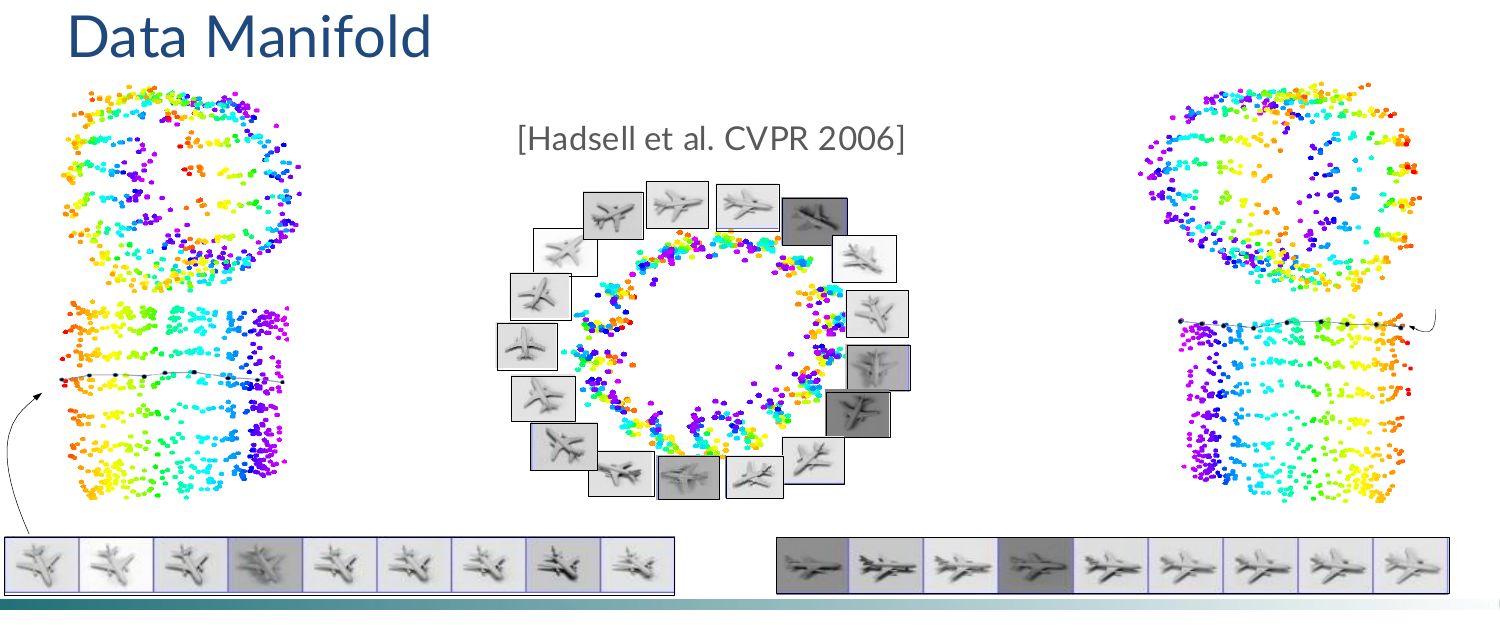
\includegraphics[width=0.88\linewidth]{figures/lr02_data_manifold.png}
  \caption{Data manifold appreso [Hadsell et al., CVPR 2006]: le immagini
           di aeroplani in diverse orientazioni formano una struttura ciclica
           coerente nello spazio di embedding -- punti vicini corrispondono a
           immagini visivamente simili.}
  \label{fig:data_manifold}
\end{figure}

%------------------------------------------------------------
\section{Architetture Multilayer = Struttura Compositiva}
\label{sec:multilayer}

I dati naturali hanno una \textbf{struttura compositiva}: sono costruiti
gerarchicamente da elementi via via più astratti. Le reti neurali multilayer
sfruttano questa struttura, con ogni layer che apprende un livello di
astrazione \citep{lecun2021}.

\begin{figure}[H]
  \centering
  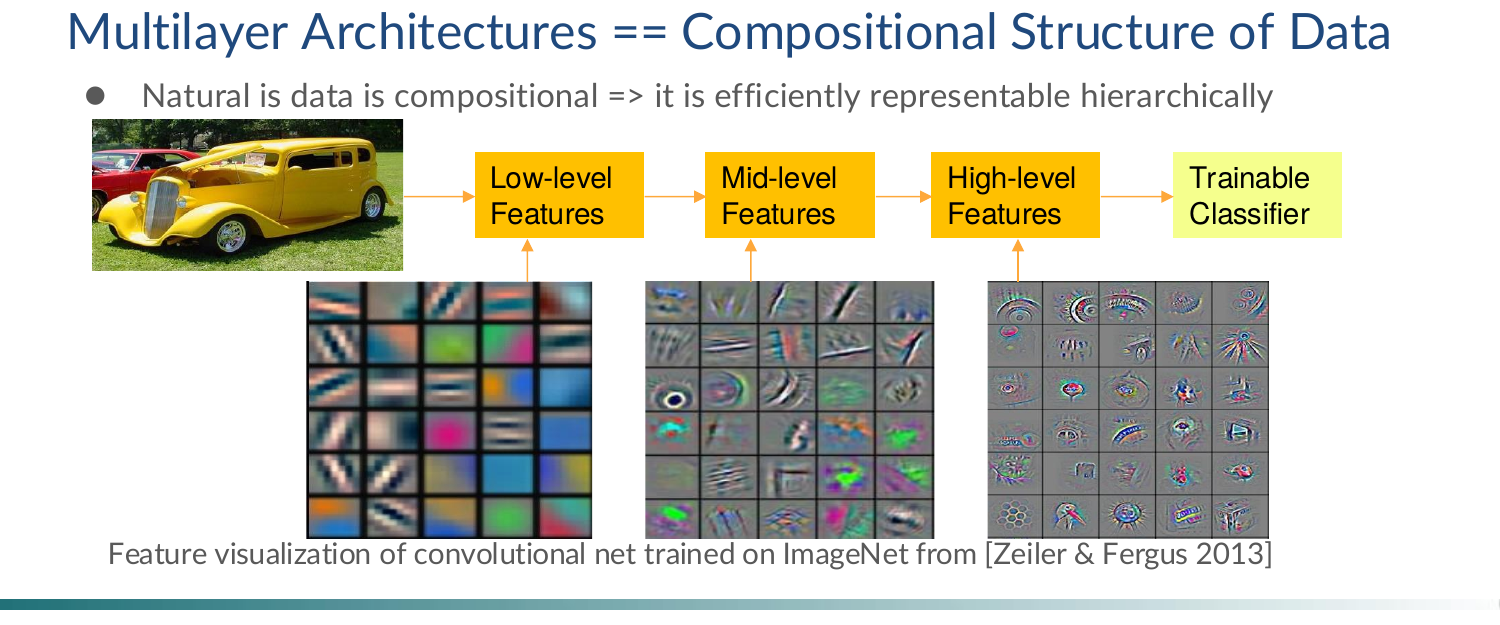
\includegraphics[width=0.92\linewidth]{figures/lr02_compositional.png}
  \caption{Le architetture multilayer corrispondono alla struttura compositiva
           dei dati. La visualizzazione delle feature di una CNN addestrata su
           ImageNet [Zeiler \& Fergus, 2013] mostra: layer bassi = edge e
           texture, layer intermedi = parti di oggetti, layer alti = concetti
           semantici.}
  \label{fig:compositional}
\end{figure}

\paragraph{Gerarchia di rappresentazioni nei diversi domini.}

\begin{figure}[H]
  \centering
  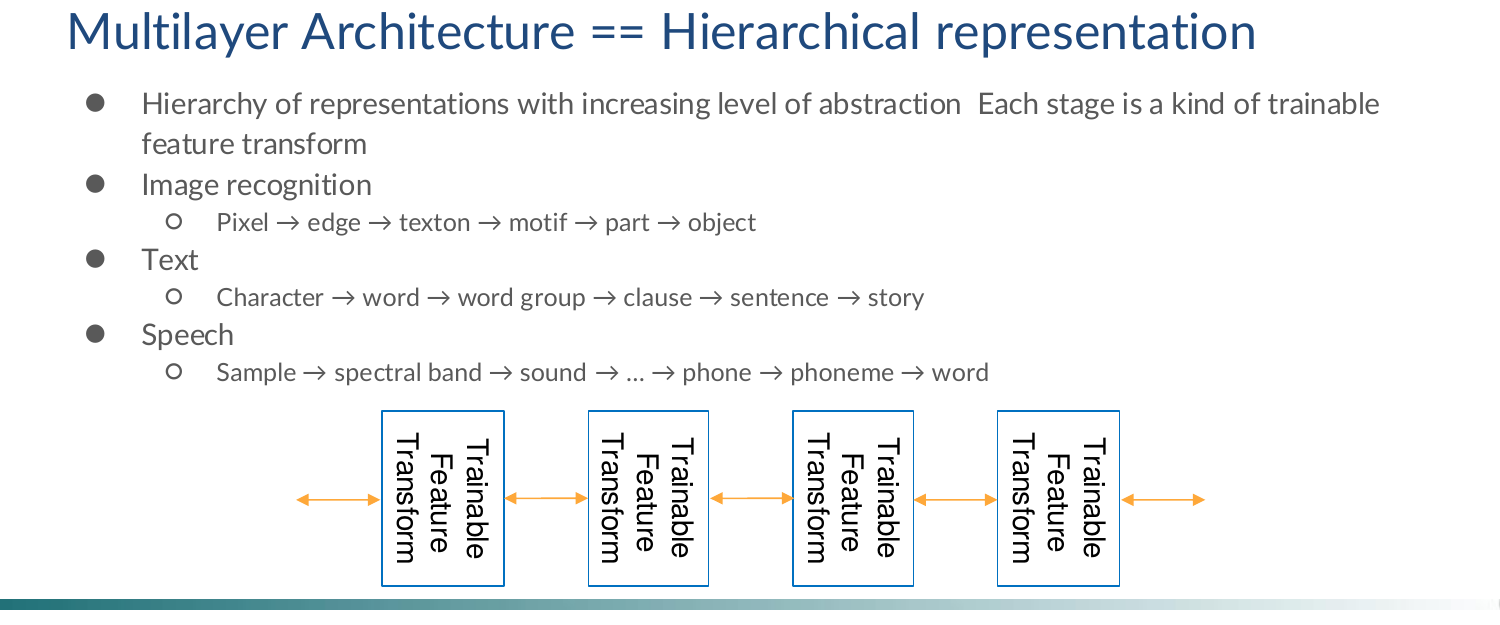
\includegraphics[width=0.82\linewidth]{figures/lr02_hierarchical.png}
  \caption{Architettura multilayer come rappresentazione gerarchica: ogni
           blocco ``Trainable Feature Transform'' corrisponde a un livello di
           astrazione. Le frecce bidirezionali indicano che ogni modulo
           può essere addestrato con backpropagation.}
  \label{fig:hierarchical}
\end{figure}

La gerarchia di astrazioni varia a seconda del dominio:
\begin{itemize}
  \item \textbf{Immagini}: pixel $\to$ edge $\to$ texton $\to$ motif
        $\to$ parte $\to$ oggetto.
  \item \textbf{Testo}: carattere $\to$ parola $\to$ gruppo di parole
        $\to$ proposizione $\to$ frase $\to$ storia.
  \item \textbf{Audio}: campione $\to$ banda spettrale $\to$ suono
        $\to$ \ldots $\to$ fonema $\to$ parola.
\end{itemize}

L'efficienza delle architetture profonde è spiegata da
\citet{lecun2021} e da Bengio \& LeCun (2007): una rete profonda
\textit{scambia ampiezza con profondità} -- più layer sequenziali ma
meno hardware parallelo -- riuscendo a rappresentare funzioni complesse
con molti meno parametri rispetto a una rete shallow.

%------------------------------------------------------------
\section{Riepilogo}
\label{sec:summary-ch2}

\begin{center}
\begin{tabular}{lll}
  \toprule
  \textbf{Concetto} & \textbf{Idea chiave} & \textbf{Implicazione} \\
  \midrule
  Classificatore lineare & $\bar{y}=\operatorname{sign}(\vect{w}^T\vect{x}+b)$ & Limite: non sep. lineare \\
  Teorema di Cover       & Prob.\ sep.\ $\to 0$ se $P \gg N$      & Serve non-linearità \\
  Feature monomiali      & Cross-products di grado $d$             & $O(N^d)$ feature \\
  Reti shallow           & Approssimatori universali               & Ma inefficienti \\
  Reti profonde          & $y = F(W^K \cdot F(\ldots))$           & Più efficienti \\
  Manifold Hypothesis    & Dati su manifold bassa-dim.             & Motiva il DL \\
  Disentangling          & Separare i fattori di variazione        & Obiettivo del repr.\ learning \\
  Struttura compositiva  & Pixel $\to$ edge $\to$ parte $\to$ obj & Giustifica i multilayer \\
  \bottomrule
\end{tabular}
\end{center}

Le reti neurali profonde sono giustificate non solo dall'approssimazione
universale (che vale anche per reti shallow), ma dalla loro
\textbf{efficienza parametrica} nel rappresentare le funzioni utili per i
compiti AI. L'ipotesi del manifold e la struttura compositiva dei dati
naturali forniscono le basi teoriche per questa efficienza.
